\begin{example}
Προσδιορίστε το μετασχηματισμό $M$ που περιστρέφει τη δοσμένη πυραμίδα $ABCD$ κατά γωνία $\theta$ ως προς το δοσμένο άξονα περιστροφής $R$.

		\begin{figure}[hbt]
		\begin{center}
		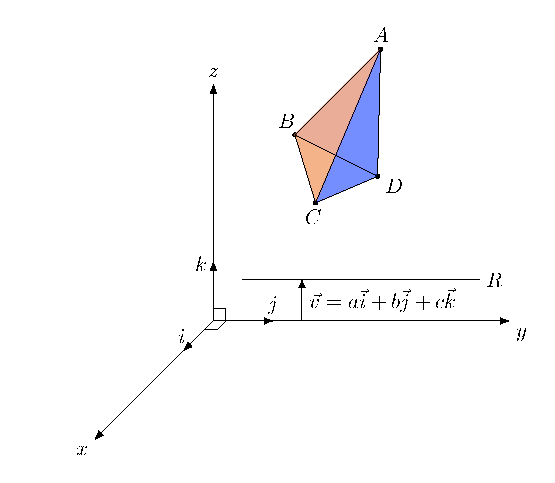
\includegraphics[scale=1]{Chapter3/example-pyramid.pdf}
		\end{center}
		\caption{Πυραμίδα $ABCD$ που ζητείται να περιστραφεί κατά γωνία $\theta$ ως προς το δοσμένο άξονα περιστροφής $R$}
		\end{figure}

\end{example}

\begin{solution}
	Παρατηρούμε ότι ο άξονας $R$ είναι παράλληλος ως προς το επίπεδο $xz$ και βρίσκεται σε απόσταση που καθορίζεται από το διάνυσμα $v$. Θα προσπαθήσουμε λοιπόν να τον ταυτίσουμε με τον άξονα των $x$. Τα ακόλουθα βήαμτα χρειάζονται για να προσδιορίσουμε τον ζητούμενο πίνακα μετασχηματισμού.

\textbf{Βήμα 1:} Μεταφορά του $R$ κατά διάνυμσα $v = -a\vec{i} - b\vec{j} - c\vec{k}$ ώστε ο άξονας περιστροφής να συμπέσει με τον άξονα των $x$

Βασικός πίνακας μετασχηματισμού $T_v$.

\textbf{Βήμα 2:} Στροφή ως προς τον άξονα των $x$ κατά γωνία $\theta$. 

Βασικός πίνακας μετασχηματισμού $R_{\theta, x}$.
 
\textbf{Βήμα 3:} Επαναφορά του $R_{-v}$ στην αρχική του θέση μεταφέροντας τον κατά διάνυσμα $-v$.

Βασικός πίνακας μετασχηματισμού $T_{-v}$.

Ο ζητούμενος μετασχηματισμός $M$ προκύπτει σα σύνθεση των παραπάνω βασικών μετασχηματισμών:

\begin{align*}
	M & = T_{-v} \circ R_{\theta, x} \circ T_v 	= 
		\begin{bmatrix}
			1 & 0 & 0 & a \\
			0 & 1 & 0 & b \\
			0 & 0 & 1 & c \\
			0 & 0 & 0 & 1
		\end{bmatrix} 
	\cdot 
		\begin{bmatrix}
			1 & 0 & 0 & 0 \\
			0 & \cos{\theta} & -\sin{\theta} & 0 \\
			0 & \sin{\theta} & \cos{\theta} & 0 \\
			0 & 0 & 0 & 1
		\end{bmatrix}
	\cdot 
		\begin{bmatrix}
			1 & 0 & 0 & -a \\
			0 & 1 & 0 & -b \\
			0 & 0 & 1 & -c \\
			0 & 0 & 0 & 1
		\end{bmatrix}  = \\
	&=	
	\begin{bmatrix}
			1 & 0 & 0 & 0 \\
			0 & \cos{\theta} & -\sin{\theta} & -b\cos{\theta} + c\sin{\theta} + b \\
			0 & \sin{\theta} & \cos{\theta} & -b\sin{\theta}-c\cos{\theta} + c \\
			0 & 0 & 0 & 1
		\end{bmatrix}  
\end{align*}

		Οι συντεταγμένες $A'B'C'D'$ της στραμμένης πυραμίδας προκύπτουν από τον ακόλουθο πολλαπλασιασμό: 
		
\[
	A'B'C'D' = M \cdot ABCD
\]		
	
\begin{remark}
	Είναι ιδιαιτέρως χρήσιμο στους μετασχηματισμούς στο χώρο των τριών διαστάσεων να μπορέσουμε να καθορίσουμε τον πίνακα μετασχηματισμού που εκφράζει τη στροφή ενός αντικειμένου ως προς ένα οποιοδήποτε δοσμένο άξονα στον χώρο. Στα επόμενα παραδείγματα αντιμετωπίζεται το συγκεκριμένο πρόβλημα.	
\end{remark}

	
\end{solution}